\documentclass{article}

% preambulo:
\usepackage[utf8]{inputenc}
% caracteres utf8 (tildes, enie) sin tener que usar comandos

\usepackage[spanish, es-tabla, es-nodecimaldot]{babel} 
% texto automatico en espaniol
% "tabla" en vez de "cuadro"
% no reemplaza puntos decimales por comas

%% NO AGREGAR PAQUETES ANTES DE ESTO, ES IMPORTANTE QUE BABEL ESTE PRIMERO

%%%%%%%%%%%%%%%%%%%%%%%%%%%%%%%%%
%% PAQUETES EXTRA %%%%%%%%%%%%%%%
%%%%%%%%%%%%%%%%%%%%%%%%%%%%%%%%%

\usepackage{subfiles}

%nuevo
\usepackage[notransparent]{svg}
%

\usepackage{amsmath} % PAQUETES DE MATEMATICA
\usepackage{amsfonts}
\usepackage{amssymb}

%puse esta cosa nueva---
\usepackage{csvsimple}

%-----
\usepackage{steinmetz} % comando \phase{}
\usepackage{units} % permite usar nicefrac
\usepackage{graphicx} % importar imagenes
\usepackage{float} % posicion H para floats
\usepackage[colorinlistoftodos]{todonotes}


\usepackage[a4paper, total={6in, 8in}]{geometry} 
% margenes correctos en subarchivos

\setlength{\parindent}{10pt}			%cuanta sangria al principio de un parrafo
\usepackage{indentfirst}				%pone sangria al primer parrafo de una seccion

\usepackage{listings}

\usepackage{color}

\definecolor{codegreen}{rgb}{0,0.6,0}
\definecolor{codegray}{rgb}{0.5,0.5,0.5}
\definecolor{codepurple}{rgb}{0.58,0,0.82}
\definecolor{backcolour}{rgb}{0.95,0.95,0.92}
 
\lstdefinestyle{mystyle}{
    backgroundcolor=\color{backcolour},   
    commentstyle=\color{codegreen},
    keywordstyle=\color{magenta},
    numberstyle=\tiny\color{codegray},
    stringstyle=\color{codepurple},
    basicstyle=\footnotesize,
    breakatwhitespace=false,         
    breaklines=true,                 
    captionpos=b,                    
    keepspaces=true,                 
    numbers=left,                    
    numbersep=5pt,                  
    showspaces=false,                
    showstringspaces=false,
    showtabs=false,                  
    tabsize=2
}
 
\lstset{style=mystyle}

%%%%%%%%%%%%%%%%%%%%%%%%%%%%%%%%%%%%%%%%%%%%%%%%%%%%%%%%%%%
%% NO AGREGAR PAQUETES DESPUES DE ESTO, ES IMPORTANTE QUE HYPERREF ESTE ULTIMO
\usepackage[hidelinks]{hyperref} % hipervinculos sin cajitas rojas
\usepackage{bm}


\begin{document}

\newgeometry{} % margenes default para la caratula
% caratula:
\begin{titlepage}
\newcommand{\HRule}{\rule{\linewidth}{0.5mm}}
\center
\mbox{\textsc{\LARGE \bfseries {Instituto Tecnol\'ogico de Buenos Aires}}}\\[1.5cm]
\textsc{\Large 22.85 - Sistemas de Control}\\[0.5cm]


\HRule \\[0.6cm]
{ \Huge \bfseries Trabajo de Laboratorio N$^{\circ}$1: Phase-Locked Loop (PLL) o Lazo de Enganche de Fase}\\[0.4cm] % Title of your document
\HRule \\[1.5cm]


{\large

\emph{Grupo 1}\\
\vspace{3px}

\begin{tabular}{lr} 	
\textsc{M\'aspero}, Martina  & 57120 \\
\textsc{Mestanza}, Joaqu\'in Mat\'ias  & 58288 \\
\textsc{Nowik}, Ariel Santiago  & 58309 \\
\textsc{Panaggio Venerandi}, Guido Martin  & 56214 \\
\textsc{Parra}, Roc\'io  & 57669 \\
\textsc{Regueira}, Marcelo Daniel  & 58300 \\

\end{tabular}

\vspace{20px}

\emph{Profesor}\\
\vspace{3px}
\textsc{Nasini}, V\'ictor Gustavo\\ 	
\vspace{100px}

\begin{tabular}{ll}

Presentado: & 27/09/2019\\

\end{tabular}

}

\vfill

\end{titlepage}

% cambio los margenes para el resto del documento
\newgeometry{left=2.5cm, top=2.5cm, right=2cm, bottom=2cm}

% indice:
\tableofcontents
\newpage

\section*{Ejercicio 1: Prelaboratorio}
\addcontentsline{toc}{section}{Ejercicio 1: Prelaboratorio}
Se pidió analizar distintas transferencias (en la sección Prelaboratorio) del diagrama en bloques del circuito provisto por la cátedra.
\begin{figure}[H]
\centering
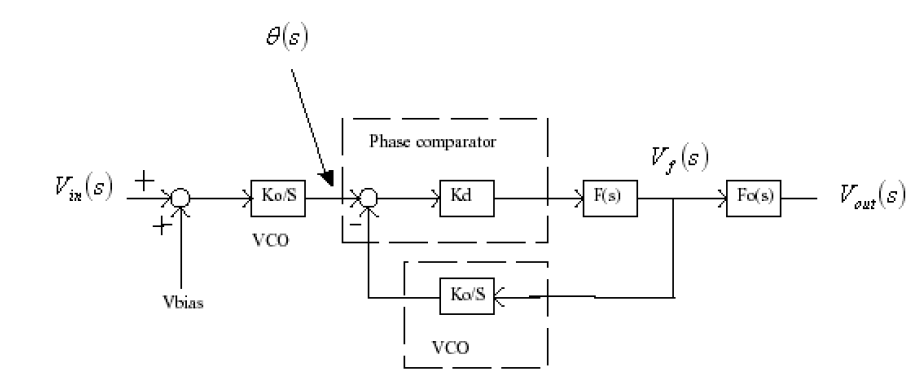
\includegraphics[width=1\linewidth]{images/Circuito.PNG}
\caption{Diagrama en bloques del circuito}
\label{fig:Circuito}
\end{figure}

\subsection*{a) Modulador (VCO)}

\begin{equation} \label{mod_eqn}
\frac{\theta(s)}{V_{in}(s)} = \frac{K_0}{s}
\end{equation}

\subsection*{b) Demodulador (PLL)}

\begin{equation} \label{demod_eqn}
\frac{V_f(s)}{\theta(s)} = \frac{s\cdot K_d \cdot F(s)}{s+K_0K_dF(s)}
\end{equation}

\subsection*{c) Filtros pasabajos: $F_1(s)$ y $F_2(s)$}

\begin{equation} \label{f1_eqn}
F_1(s) = \frac{1}{ 1 + \frac{s}{\omega_1}
}
\qquad \text{donde} \qquad \omega_1=\frac{1}{R_5\cdot C_6} 
\end{equation}


\begin{equation} \label{f2_eqn}
F_2(s) = \frac{1+\frac{s}{\omega_2}}{ 1 + \frac{s}{\omega_{eq}}} \qquad \text{donde} \qquad \omega_2=\frac{1}{R_6\cdot C_6} \qquad \omega_{eq} = \frac{1}{\frac{1}{\omega_1} + \frac{1}{\omega_2}} 
\end{equation}


\subsection*{d) $F_0(s)$}

\begin{equation} \label{fo_eqn}
F_0(s) = \frac{V_{out}(s)}{V_f(s)} = \frac{1}{ 1 + \frac{s}{\omega_0}} \qquad \text{donde} \qquad \omega_0=\frac{1}{R_9\cdot C_7}
\end{equation}

\newpage

\section*{Ejercicio 2: Factor de amortiguamiento considerando los filtros}
\addcontentsline{toc}{section}{Ejercicio 2: factor de amortiguamiento considerando los filtros}

Notar que lo que cambia entre los filtros es $R_6$, así que dejamos las expresiones generales.

\begin{equation} \label{vftheta_eqn}
\frac{V_f(s)}{\theta(s)} = \frac{ s}{K_0}
\cdot \frac{ 1 + \frac{s}{\omega_2} }
{ \left(\frac{s}{\omega_n}\right)^2 + 2\frac{\xi}{\omega_n}  + 1}
\end{equation}

\begin{equation} \label{wn_eqn}
\omega_n = \sqrt{\frac{K_d K_0}{C_6\cdot(R_5+R_6)}}
\end{equation}


\begin{equation} \label{xi_eqn}
\xi = \frac{R_6 \cdot C_6\cdot K_d\cdot K_0  + 1}
{2\cdot \sqrt{C_6 \cdot K_d \cdot K_0 \cdot(R_5 + R_6)}}
\end{equation}

\section*{Ejercicio 3: Transferencia completa}
\addcontentsline{toc}{section}{Ejercicio 3: Transferencia completa}

\begin{equation} \label{voutvin_eqn}
\frac{V_{out}(s)}{V_{in}(s)} = \frac{V_{out}(s)}{V_f(s)} \cdot \frac{V_f(s)}{\theta(s)}\cdot \frac{\theta(s)}{V_{in}(s)}
\end{equation}

\begin{equation} \label{voutvin_eqn_posta}
\frac{V_{out}(s)}{V_{in}(s)} = \frac{1}{ 1 + \frac{s}{\omega_0}} 
\cdot \frac{ 1 + \frac{s}{\omega_2} }
{ \left(\frac{s}{\omega_n}\right)^2 + 2\frac{\xi}{\omega_n}  + 1} 
\end{equation}

\newpage

\section*{Laboratorio}
\addcontentsline{toc}{section}{Laboratorio}
Para poder simular la transferencia completa se necesitan hallar los valores $K_0$ y $K_d$.
Para esto, se procedió inyectar una entrada de tensión continua a la entrada del VCO, variando su valor en el rango de 1V a 10V. Con eso se obtuvo la siguiente tabla:
\begin{table}[H]
	\centering
	\label{table7}
	\begin{tabular}{c c c c c}%
		\bfseries \# & $\bm{DC_{IN}(V)}$ & $\bm{freq_{out}(KHz)}$ & $\bm{K_0(rad/seg/V)}$  \\ \hline
		\csvreader[head to column names, late after line=\\]{vco.csv}{}{\thecsvrow & \dc & \f & \k}
		%DC_IN(V),freq_out(KHz),K0 ((rad/seg)/V)
		\hline
	\end{tabular}
		\caption{Tabla centrada con datos obtenidos}
\end{table}

Como se solicita ingresar al VCO con una señal de 0.5 Vpp y además un offset de 5V, se le da un peso mayor a las mediciones 4, 5 y 6. Con este  criterio, se optó por un valor para $K_0$ de:
\[ K_0= 1M \left[\frac{rad \cdot seg}{V}\right] \]

Luego, para determinar la constante $K_d$ se consultó la datasheet del CD4046 de Texas Instruments. En la misma se halló el siguiente gráfico:
\begin{figure}[H]
\centering
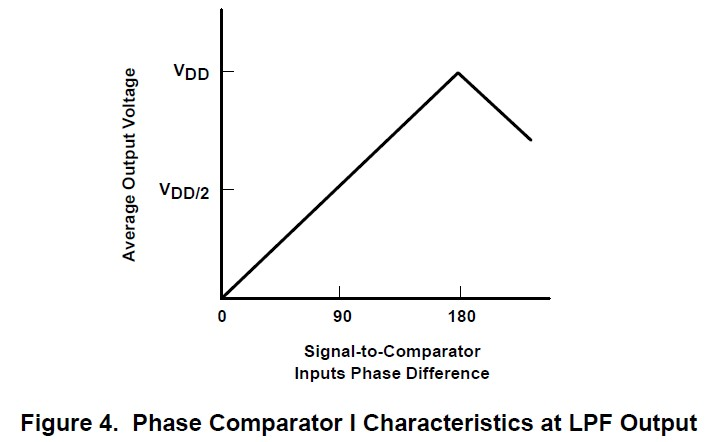
\includegraphics[width=0.6\linewidth]{images/Kd.jpg}
\caption{Características del comparador de fase tipo 1 (XOR)}
\label{fig:comp1}
\end{figure}
Por simple inspección nos queda como resultado
\[ K_d= \frac{V_{DD}}{\pi} \left[\frac{V}{rad}\right] \]
Con estos valores y los establecidos por la consigna podemos calcular $\xi$ y $\omega_n$ para cada caso:
\[ \xi = 0.0886 \qquad \text{donde} \qquad \omega_n = 5.6419\cdot 10^{5} \left[\frac{rad}{seg}\right] \qquad (RC) \]
Mediante el despeje de la ecuación \ref{xi_eqn} se halló que para que $\xi \approx 0.5$ se necesita una $R_6 = 1.6K\Omega$
\[ \xi = 0.5014 \qquad \text{donde} \qquad \omega_n = 5.2384\cdot 10^{5} \left[\frac{rad}{seg}\right] \qquad (RRC) \]


\newpage
\section*{Mediciones: Filtro con F1 - Caso RC}
\addcontentsline{toc}{section}{Mediciones: Filtro con F1 - Caso RC}

\begin{figure}[H]
\centering
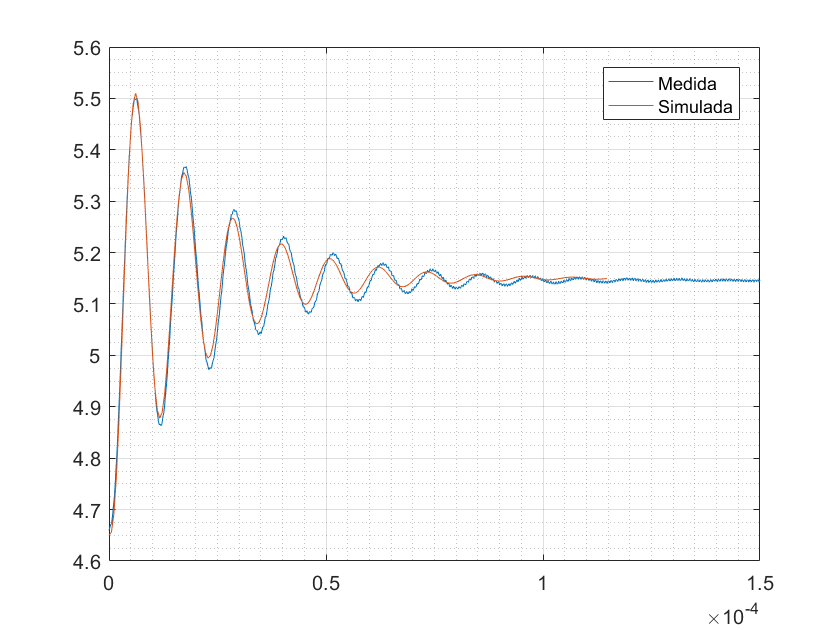
\includegraphics[width=0.8\linewidth]{images/conF1_superpuestas.PNG}
\caption{Mediciones superpuestas con la curva teórica - Caso RC}
\label{fig:superpF1}
\end{figure}




\begin{figure}[H]
\centering
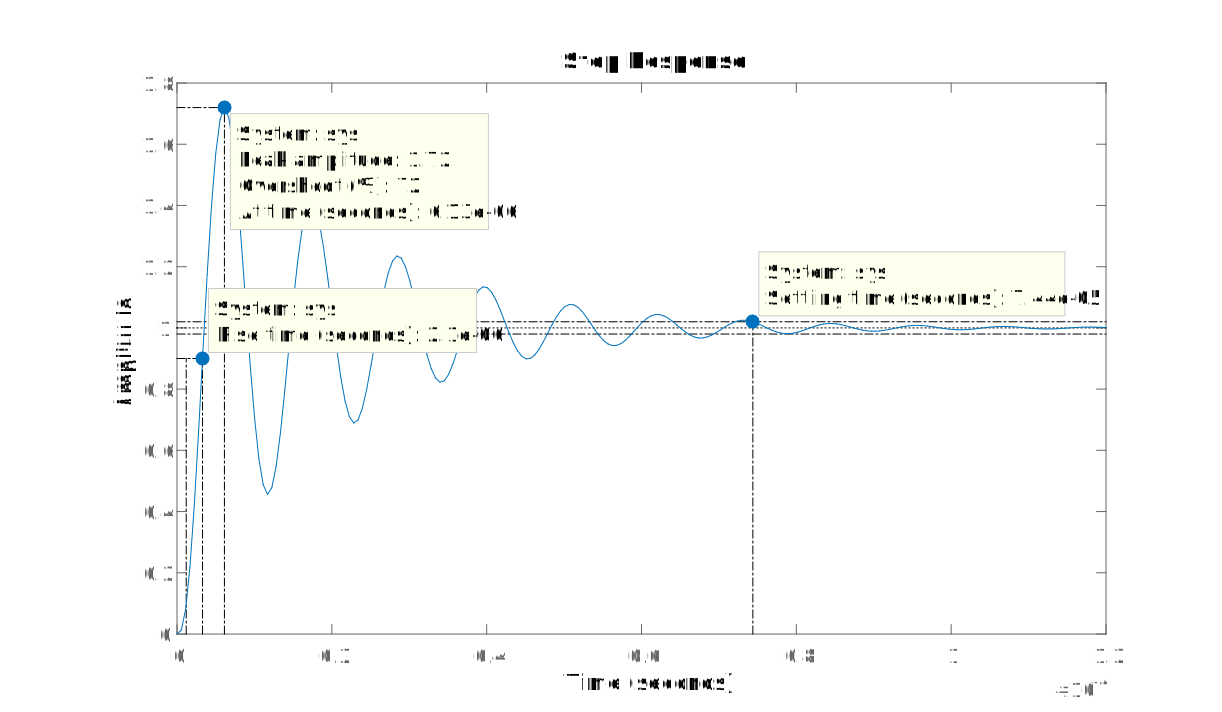
\includegraphics[width=1\linewidth]{images/todo.PNG}
\caption{Simulaciones con el filtro RC}
\label{fig:sim}
\end{figure}

\begin{figure}[H]
\centering
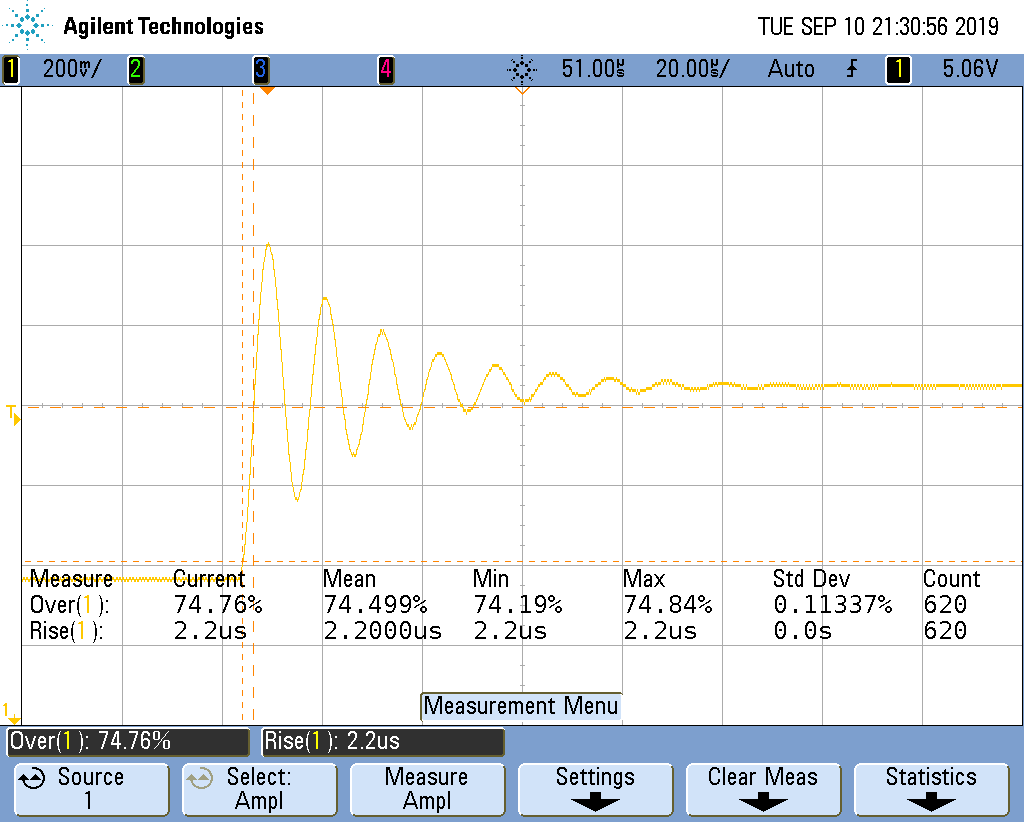
\includegraphics[width=0.8\linewidth]{images/os_and_trise.PNG}
\caption{Mediciones: Overshoot y Rise Time}
\label{fig:osandtr}
\end{figure}

\begin{figure}[H]
\centering
\includegraphics[width=0.8\linewidth]{images/tpeak_vpeak.PNG}
\caption{Mediciones: Peak Value y Peak Time}
\label{fig:peak}
\end{figure}

\begin{figure}[H]
\centering
\includegraphics[width=0.8\linewidth]{images/settling_time.PNG}
\caption{Mediciones: Settling Time}
\label{fig:ts}
\end{figure}

\newpage

\section*{Mediciones: Filtro con F2 - Caso RRC}
\addcontentsline{toc}{section}{Mediciones: Filtro con F2 - Caso RRC}

\begin{figure}[H]
\centering
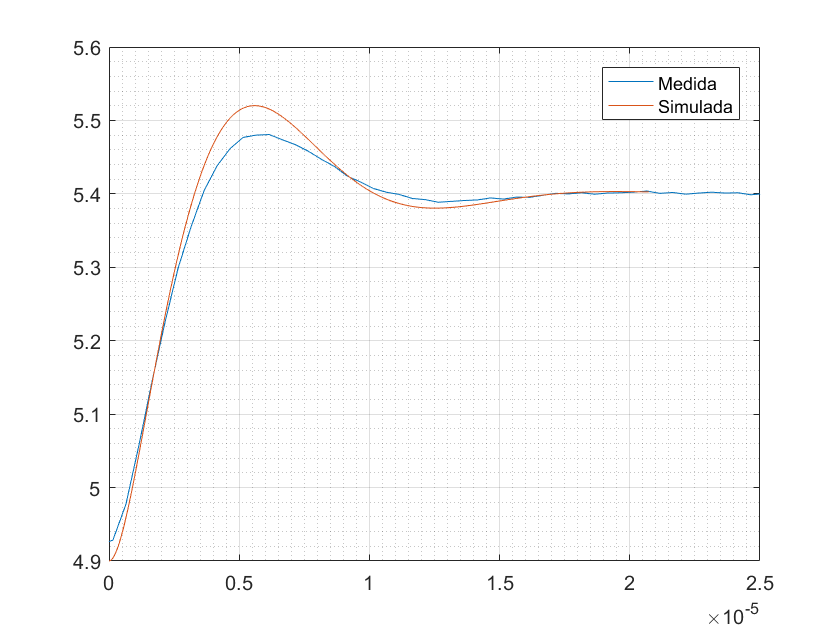
\includegraphics[width=0.8\linewidth]{images/conF2_superpuestas05.PNG}
\caption{Mediciones superpuestas con la curva teórica - Caso RRC}
\label{fig:superpF2}
\end{figure}

\begin{figure}[H]
\centering
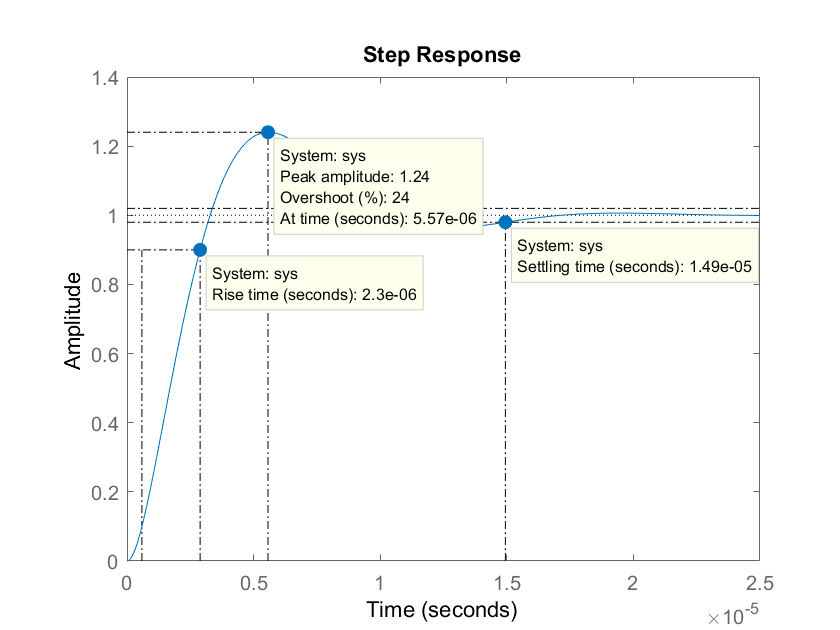
\includegraphics[width=0.8\linewidth]{images/05vpp/simu.PNG}
\caption{Simulaciones con el filtro RRC}
\label{fig:simu}
\end{figure}


\begin{figure}[H]
\centering
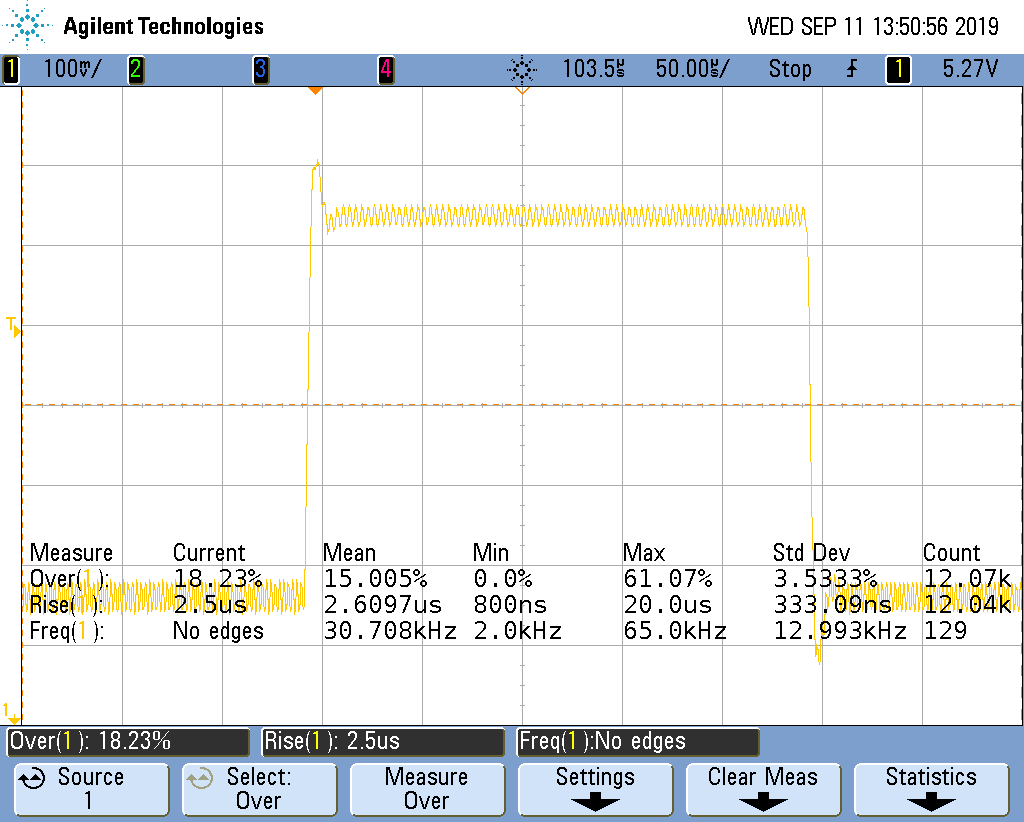
\includegraphics[width=0.8\linewidth]{images/05vpp/os_rt05vpp.PNG}
\caption{Mediciones: Overshoot y Rise Time}
\label{fig:os_rt05vpp}
\end{figure}

\begin{figure}[H]
\centering
\includegraphics[width=0.8\linewidth]{images/05vpp/tpeak_vpeak.PNG}
\caption{Mediciones: Peak Value y Peak Time}
\label{fig:tpeak_vpeak}
\end{figure}


\begin{figure}[H]
\centering
\includegraphics[width=0.8\linewidth]{images/05vpp/settling_time.PNG}
\caption{Mediciones: Settling Time}
\label{fig:settling_time}
\end{figure}


\section*{Filtro de salida}
\addcontentsline{toc}{section}{Filtro de salida}
Dado que a la salida del comparador de fase del sistema PLL presenta cambios abruptos, al ir conectada a la entrada del VCO se terminan traduciendo en cambios abruptos en la frecuencia de la señal de salida del VCO (dado que la misma varía con la tensión a su entrada). Por este motivo, entre medio de ambos bloques se coloca un filtro pasabajos para suavizar dichos cambios. Para implementarlo se presentaron dos opciones (RC y RRC), obteniendo resultados que muestran diferencias claras entre ambos:\par
En el caso del RC, se logran filtrar las altas frecuencias satisfactoriamente, pero no termina permitiendo modificar el factor de amortiguamiento. En cambio, el caso con RRC permite modificar el factor de amortiguamiento, pero al ser una transferencia que mantiene la forma pasabajos hasta un determinado valor y luego se vuelve constante, las altas frecuencias terminan ingresando (aunque más atenuadas).

Desde un punto de vista teórico esta etapa no afecta la transferencia del PLL propiamente dicho, ya que se localiza a la salida de éste, pero si tiene influencia en la transferencia del sistema total. Según los valores propuestos por la cátedra para el resistor y el capacitor se tiene que la constante de tiempo es de 560ns. Dicha constante afecta de forma significativa el sistema ya que cuanto menor sea esta menor es el tiempo que demora el sistema en que la señal de salida alcance el valor final, pero mayor será su ancho de banda, y viceversa.
A modo de comparación se muestran los resultados característicos obtenidos en cada caso.

\begin{table}[H]
	\centering
\begin{tabular}{|c|c|c|c|c|}
\hline
\multicolumn{2}{|c|}{}                & Overshoot (\%) & Rise Time & Settling Time \\ \hline
\multirow{2}{*}{Filtro RC}  & Teórico & 0.72           & 2.1 us    & 74.4 us       \\ \cline{2-5} 
                            & Medido  & 0.74           & 2.2 us    & 81 us         \\ \hline
\multirow{2}{*}{Filtro RRC} & Teórico & 0.24           & 2.3 us    & 14.9 us       \\ \cline{2-5} 
                            & Medido  & 0.18           & 2.5 us    & 12.5 us       \\ \hline
\end{tabular}
	\caption{Tabla centrada con datos característicos}
\end{table}

\newpage

\section*{Conclusiones}
\addcontentsline{toc}{section}{Conclusiones}
Se ha estudiando el proceso de diseño y las bases teóricas que sostienen el funcionamiento del PLL. Las pruebas realizadas sobre el mismo consistieron fundamentalmente en observar y analizar la respuesta dinámica del sistema al escalón realizando una comparación con los cálculos teóricos previos y las simulaciones hechas, para los distintos filtros sugeridos.\par
Observando los resultados obtenidos, se deja en evidencia que cada filtro proporciona una ventaja particular permitiendo controlar un determinado parámetro del sistema, pero no pudiendo modificar otro, como se analizó previamente sobre la etapa del filtrado de la salida. Con todo lo anterior se pudo analizar y observar correctamente el funcionamiento del PLL como un sistema del control realimentado el cual entre otras cosas permitirá realizar la demodulacion de una señal de FM, dados los parámetros de trabajo adecuados, debido a dicho control que se realiza sobre la señal.

\end{document}
